\chapter{Metodologia}
\label{cap:metodologia}
 Apresentamos neste capítulo a nossa proposta de visualização para exploração
dos fluxos no tráfego de veículos. O objetivo principal da visualização é centrado
nas propriedades espaciais e temporais dos dados para entender
como os fluxos se deslocam pela cidade ao longo do tempo. Buscamos
um maior nível de detalhes através de uma abordagem multinível para
explorar padrões globais e locais do tráfego, com diferentes níveis de agregação
temporais e espaciais.

 Apresentamos inicialmente os conjuntos de dados
utilizados e suas características. Então, explicamos o projeto da visualização
com as técnicas que pretendemos utilizar para destacar as propriedades dos dados,
e por fim, damos alguns detalhes sobre a implementação da ferramenta de visualização
InterSCityPlot.

\section{Conjuntos de Dados}
   Os dados do tráfego que utilizaremos possuem o registro da posição ao longo
de toda a trajetória, desde a origem até seu destino. Dentre as informações
espaciais e temporais, esses conjuntos de dados usualmente também apresentam
outras características, como direção e velocidade, formando um conjunto
multidimensional. Cada trajetória $T$ de um veículo pode ser modelada como uma
sequência de pontos $p_i$ que contém a sua posição, o instante de tempo e um
vetor de possíveis outros atributos.

\begin{center}
$T = \left\langle p_i = ((latitude, longitude) \in \mathbb{R}^2, t \in \mathbb{R}^+, a^n \in \mathbb{R})_i \right\rangle$
\end{center}

  Duas fontes de dados com informações do tráfego de veículos na cidade de São
Paulo serão usadas neste trabalho. A primeira é uma API pública disponibilizada
pela prefeitura da cidade e que fornece dados da movimentação dos ônibus. A
outra fonte é o simulador InterSCSimulator, o qual usaremos para obter dados
do tráfego.

\subsection{Tráfego dos Ônibus de São Paulo}
São Paulo possui uma frota de  cerca de 15 mil ônibus que circulam diariamente
nas vias da cidade e fazem mais de 70 mil viagens por dia. A posição dos ônibus
durante seu percurso é registrada a cada 45 segundos com aparelhos de GPS e
disponibilizada através de API pública. Os dados trazem o código da linha do
ônibus, horário da coleta, a latitude e longitude, entre outras informações
simples que não utilizaremos. A lista completa dos atributos podem ser vista na
documentação da API que fornece os dados. Outros atributos, como direção e
velocidade podem ainda ser calculados a partir das informações existentes.

Para a visualização do tráfego serão coletados os dados de um dia do tráfego
de ônibus. Embora não representem a totalidade do tráfego, esses dados compõe uma
grande parte da movimentação que ocorre na cidade ao longo do dia e servem como
uma linha de base para comparação com a visualização dos dados simuladas. A partir
da visualização desses dados, pretendemos descobrir os padrões de movimentação
no trânsito, como identificar regiões de maior fluxo e como ele se distribui ao longo
do tempo.

\subsection{Tráfego Simulado de Veículos}
 \citet{santana2018courb} criaram um cenário de simulação do tráfego de carros
e ônibus na cidade de São Paulo. Eles utilizaram uma matriz de Origem-Destino
(OD) feita pela Companhia do Metropolitano de São Paulo
(Metrô)\footnote{Pesquisa Origem-Destino - \rurl{goo.gl/DNM8in}} que pesquisou
como os cidadãos se locomovem pela cidade e usaram isso para determinar a
movimentação dos carros. Além disso, utilizaram também dados públicos da
Secretaria de Transporte Público (SPTrans)\footnote{\rurl{colocarurl}} para
estabelecer viagens de ônibus mais realistas com base nos dados sobre as
linhas, horários de saída, paradas e sua frequência.

  A pesquisa OD catalogou 160 mil amostras de viagens realizadas em um dia de
semana da cidade de São Paulo. Ela capta dados como a origem, o destino, a hora
de início, o modo de transporte e um fator para a extrapolação de cada viagem.
Destas viagens, cerca de 26 mil são feitas de carro, como mostram
\citet{santana2018courb}. Utilizando o fator de extrapolação da pesquisa, eles
chegam a uma quantia de mais de 4 milhões de viagens de carro e ônibus em um
dia, as quais foram simuladas com o InterSCSimulator.

  A simulação gerou uma saída com mais de 31 milhões de eventos sobre a
movimentação dos veículos na cidade.  Cada evento contém informações básicas:
id do veículo, horário, posição (latitude e longitude) e tipo de evento do
veículo na simulação (início, movimento ou chegada). A Tabela
\ref{table:output} mostra uma parte do arquivo de saída com os eventos gerados.
O tempo da simulação corre em segundos e dura 24 horas, ou seja, 86399
segundos.  Note que os últimos registros mostram veículos que não chegaram ao
seu destino pois a simulação foi finalizada ao fim das 24 horas.


\begin{table}[!htb]
\centering
\begin{tabular}{|c|c|c|c|c|}
\hline
\textbf{Horário} & \textbf{Ação} & \textbf{ID} & \textbf{Latitude} & \textbf{Longitude} \\
\hline
25 & start & 4858\_52 & -23.624235 & -46.648388 \\
27 & start & 4858\_73 & -23.624235 & -46.648388 \\
27 & start & 94\_17 & -23.535976 & -46.63561    \\
31 & move & 4858\_52 & -23.624077 & -46.648453 \\
33 & move & 4858\_73 & -23.624077 & -46.648453 \\
35 & start & 8394\_43 & -23.561275 & -46.695423 \\
... & ... & ... & ... & ... \\
233 & arrival & 8062\_64 & -23.567131 & -46.68642 \\
... & ... & ... & ... & ... \\
86399 & move & 9548\_87 & -23.630016 & -46.627766 \\
86399 & move & 9548\_89 & -23.613354 & -46.65802 \\
86399 & move & 9548\_92 & -23.602781 & -46.65138 \\
\hline
\end{tabular}
\caption{Resultado parcial da simulação. Fonte: \citet{santana2018courb} \label{table:output}}
\end{table}

\section{Visualização do Tráfego de Veículos}

  Apresentamos a seguir as técnicas para exploração das propriedades temporais
e espaciais dos dados em diferentes níveis de detalhes. Algumas técnicas se
inspiram em soluções apresentadas em outros trabalhos relacionados e algumas
outras surgiram a partir das necessidades desta pesquisa.

\subsection{Propriedades Temporais}
O tráfego é um ambiente altamente dinâmico que varia ao longo do
dia, principalmente em horários de pico, tendo horários de máximo fluxo em
períodos do começo da manhã e ao fim da tarde. A análise dos fluxos ao
longo do tempo é importante para identificar mudanças e eventos que alteram o
comportamento do trânsito durante um certo período. Neste sentido, permitimos
controle da dimensão temporal através de dois parâmetros, $t_{atual}$ e
$\Delta~t$, similar ao definido por \citet{Klein2013}. A combinação dos
parâmetros definem um filtro que funciona como um referência para selecionar um
conjunto de trajetórias  ${T}$ que contenham pontos dentro do intervalo
$t_{atual} + \Delta~t$, determinando uma janela de tempo. Valores de $\Delta~t$
pequenos ou nulos acabam por selecionar os pontos instantâneos das trajetórias
no instante de tempo definido por $t_{atual}$, enquanto valores maiores trazem
os demais pontos ao longo do tempo. Com isso conseguimos um alcance multi
escala dentro da dimensão temporal, permitindo a seleção de momentos
instantâneos e também de um conjunto de pontos ao longo de um grande intervalo.

\subsection{Propriedades Espaciais}

\textbf{Visualização baseada em mapa:} a representação das trajetórias em um
leiaute de linhas sobre um mapa mostra intuitivamente as relações de OD entre
as regiões da cidade em um determinado instante de tempo. Com essa projeção, as
informações espaciais são o destaque, já que ela mapeia diretamente a dimensão
espacial. A Figura \ref{fig:simulated-traffic} mostra uma simples visualização das
trajetórias do tráfego simulado com o InterSCSimulator. Utilizamos dados no
intervalo de 1 hora do trânsito filtrando os dados cujos pontos estivessem
entre os tempos $21600$ e $25200$, o que corresponde ao horário entre 6 e 7 da
manhã. Note que há bastante oclusão, sendo impossível distinguir rotas com
direções opostas ou identificar a quantidade de veículos nas vias.

\begin{figure}[!htb]
  \centering
  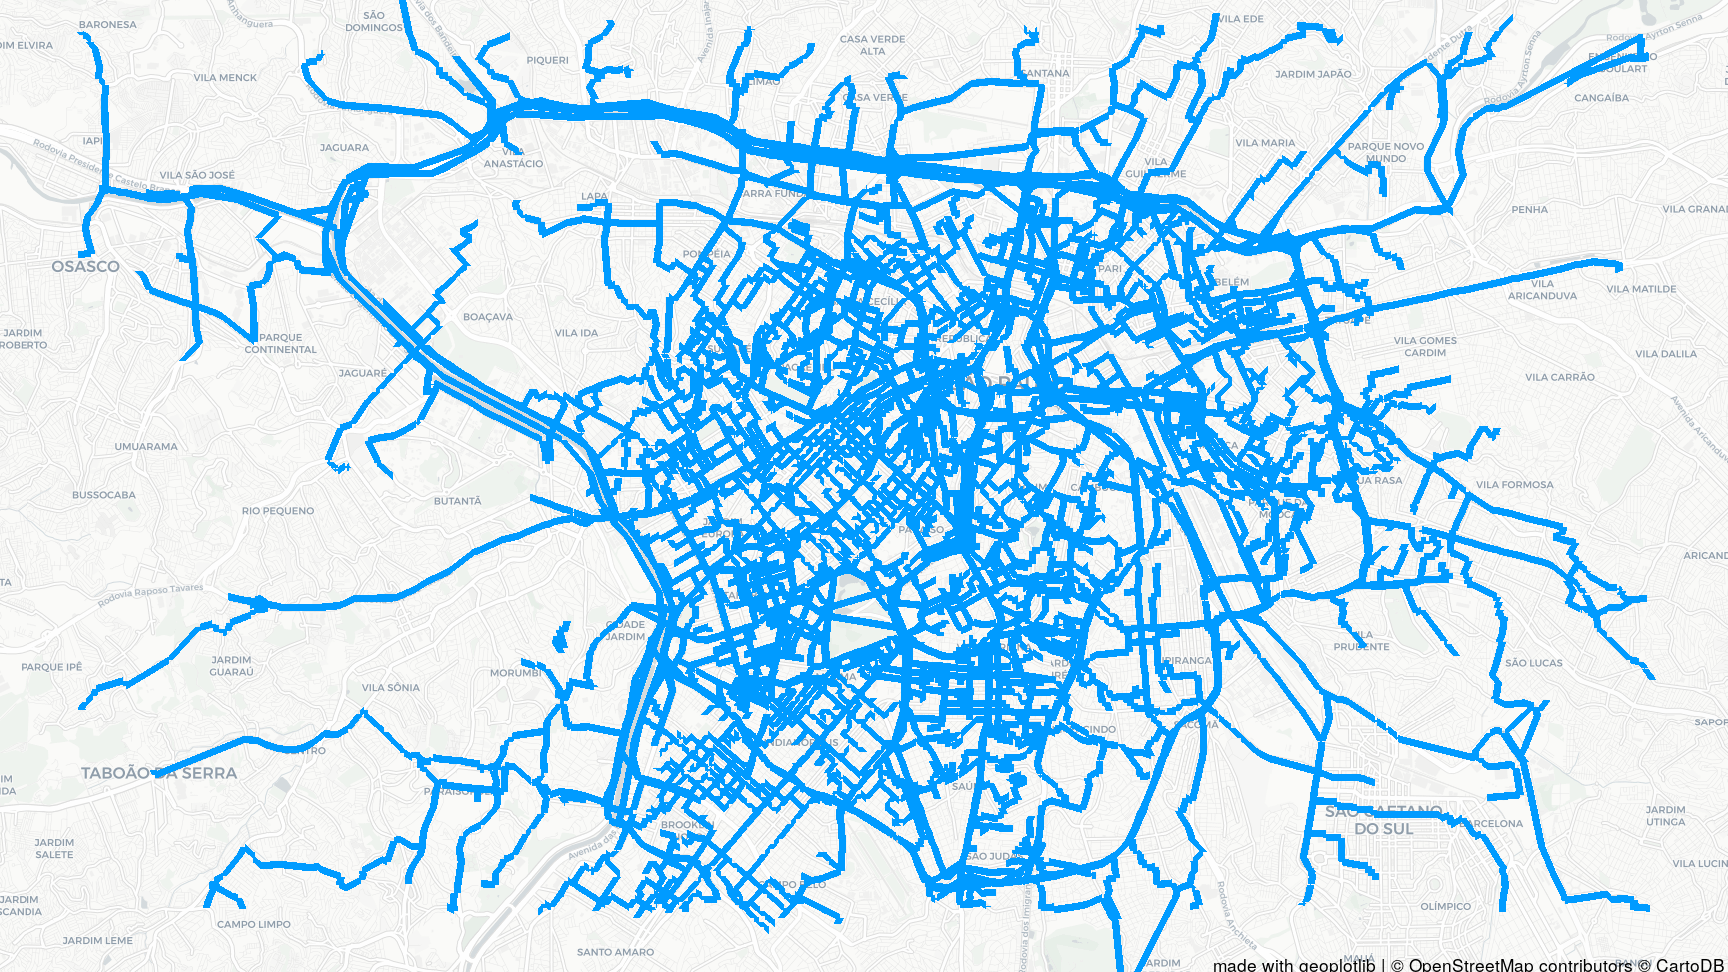
\includegraphics[width=1\textwidth]{../figuras/trafego-ocluso.png}
  \caption{Simulação do tráfego entre 6 e 7 da manhã.}
  \label{fig:simulated-traffic}
\end{figure}

\textbf{\emph{Bundling}:} para os problemas da visualização apresentados
anteriormente criaremos uma abstração com o uso do \emph{bundling} para agregar
trajetórias com origem-destino e direção similares. Já o número de trajetórias
em cada \emph{bundle} nos dá a informação da densidade do fluxo. Na escala da
cidade, as linhas dos \emph{bundles} podem demonstrar viagens de longa
distância ou desvios realizados por alguns veículos, sugerindo melhorias no
projeto da rede rodoviária.

\textbf{\emph{Bundling} Multinível:} a dimensão espacial dos dados é o nosso
segundo parâmetro multi escala dentro da visualização. Para observar os padrões
de OD em diferentes níveis de detalhe espaciais faremos agrupamentos baseados
na escala da visualização, que está relacionada ao tamanho da área do mapa
mostrada na imagem. Este mecanismo é comumente visto em visualizações
interativas que permitem aos usuários mudar as configurações de zoom no mapa. A
partir daí, é possível detectar os pontos das trajetórias dentro da área
visualizada e em seguida aplicamos o \emph{bundling}. Quanto menor a escala,
mais detalhes sobre o tráfego, que pode chegar ao nível de bairros, quadras ou
até mesmo ruas. A Figura \ref{fig:multi-scale} ilustra os diferentes níveis de
detalhe atingidos em escalas diferentes na visualização de um mapa.

\begin{figure}[!htb]
  \centering
  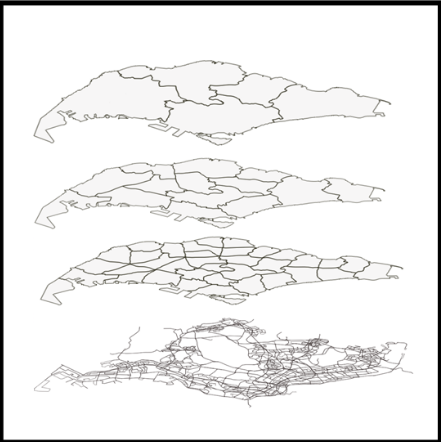
\includegraphics[width=55mm]{../figuras/multi-scale.png}
  \caption[Visualização de um mapa em diferentes escalas espaciais]{Visualização de um mapa em diferentes escalas espaciais. Fonte: \citet{Zeng2013}}
  \label{fig:multi-scale}
\end{figure}

\textbf{Parâmetros:} Grande parte dos algoritmos de \emph{bundling} possuem
parâmetros que devem ser calibrados de acordo com o contexto de uso do
algoritmo. \citet{Lhuillier2017} cita ainda que esse é ainda um grande desafio
na área, já que não existem parâmetros ideais para todo tipo de aplicação. O
CUbu, por exemplo, apresenta quatro parâmetros, raio do kernel $p_r$, número de
interações do \emph{bundling} $p_n$, resolução da imagem $p_i$ e número de
pontos de amostra $p_s$. Esses parâmetros afetam diretamente o grau de
agrupamento e o desempenho do algoritmo. Outro parâmetro importante em nossa
visualização é a escala espacial para variação do nível de detalhes do
\emph{bundling}. Esse parâmetro age como um filtro, selecionando apenas os pontos
dentro da área visualizada.

\subsection{Visualização dos Atributos}
Depois de calcular o \emph{bundling} das trajetórias, é necessário projetar uma
maneira de mostrar a estrutura dos elementos e seus atributos. Destacamos
diretamente na visualização os atributos de densidade e direção do fluxo.

\textbf{Densidade}: a densidade do fluxo é uma informação importante na análise
do fluxo. Essa informação dá uma visão sobre a quantidade de veículos se
locomovendo de uma região para outra. Esse atributo é comumente destacado de
duas formas principais, uma escala de cores, como um mapa de calor, ou através
da espessura da linha. Escolhemos escalar a espessura da linha dos
\emph{bundles} proporcionalmente à densidade do fluxo que ele representa.
Deixamos a coloração para demonstrar a direção das trajetórias, já que é uma
forma mais intuitiva para esse atributo.

\textbf{Direção}: como em \citet{Anita2017}, nos destacamos a direção das
trajetórias com um mapa de cores que indica se a trajetória está chegando ou
saindo de um ponto no mapa. É necessário ainda um cuidado com a sobreposição de
trajetórias paralelas que vão em direções opostas. \citet{Anita2017} resolvem
esse problema criando um parâmetro de repulsão para deslocar as trajetórias na
visualização, deixando mais clara a sua diferenciação.

\subsection{Visualização Interativa}

Mecanismos de interação são um excelente recurso em uma visualização de dados.
Mais do que apenas informar, os usuários podem buscar seus próprios padrões e
explorar o conteúdo à sua maneira. Adicionamos alguns meios de interação para
facilitar o estudo das trajetórias e exploração das suas propriedades.
 
\textbf{Parâmetros:} Todos os parâmetros mencionados anteriormente para a exploração
multinível no tempo e no espaço serão configuráveis para os usuários da visualização,
bem como os parâmetros do algoritmo de \emph{bundling}. Desta maneira ganha-se
a liberdade para seleção dos parâmetros que melhor se adequam aos objetivos
da visualização.

\textbf{Inspecionando os \emph{bundles}}: analisando-se um \emph{bundle},
podemos dar ainda mais detalhes sobre as trajetórias que o formam para
responder duas questões importantes para análise dos fluxos: 'Qual o percentual
das trajetórias veem de uma determinada região?' ou 'Qual região é maior
responsável pelo fluxo naquele trecho?'.  Essa informação pode ser obtida
observando-se a composição do \emph{bundle} e oferece mais detalhes para que
gestores da cidade entendam melhor a estrutura do trânsito e as relações de OD.

 Para inserir esse dado na visualização recorremos a uma nova
imagem, disparada pela interação do usuário que poderá inspecionar um
\emph{bundle} para visualizar esses detalhes em uma caixa de diálogo com as
estatísticas percentuais sobre as origens das trajetórias.

\section{Correlação com Eventos Externos}

  Outra importante tarefa na análise do trânsito é o estudo de como a
ocorrência de eventos externos impactam no tráfego. Para essa tarefa, propomos
a utilização de dados que representem diferentes cenários do trânsito para
explorar como a visualização proposta ajuda na identificação desses eventos
atípicos no trânsito e como eles afetam o tráfego. Para isso, faremos uma
simulação com o InterSCSimulator e bloquearemos vias importantes da cidade por
onde passam uma grande quantidade de veículos de diversas regiões, como por
exemplo a Avenida Paulista. Esperamos que o bundling revele as alterações nos
padrões de deslocamento dos veículos e que esses sejam visualmente
perceptíveis. Avaliar esse tipo de cenário é importante para demonstrar como a
técnica pode ajudar em questões do dia a dia no trânsito, como a ocorrência de
acidentes, alagamentos e mudanças na rede rodoviária da cidade.

\section{Avaliação da Visualização}
  Nós avaliamos a visualização de dois pontos de vista, um qualitativo e um
quantitativo. Do ponto de vista qualitativo apontaremos o que foi alcançado com
a visualização em relação os objetivos da pesquisa de utilizar técnicas de \emph{bundling}
para visualização dos fluxos de OD no tráfego. Avaliaremos então se a visualização
tornou possível a visualização dos fluxos de OD nos diferentes níveis de
detalhe e quais foram suas limitações. Além disso, analisamos também o potencial da
visualização com \emph{bundling} em representar mudanças no trânsito na
ocorrência de eventos externos, tais como o fechamento de uma rua importante do
tráfego. Dentre essas avaliações, serão experimentados os diferentes parâmetros
do algoritmo de \emph{bundling} e das técnicas de visualização utilizadas, com
uma caracterização sobre quais valores dos parâmetros foram considerados mais adequados.

  Do ponto de vista quantitativo pretendemos avaliar a escalabilidade da
solução dado o tempo de processamento para gerar a visualização de um certo
conjunto de dados. Para isso, iremos contar o tempo para gerar a visualização
ignorando etapas de pré-processamento e carregamento dos dados. 

\section{Implementação da Visualização}
  Apresentamos o InterSCityPlot, uma ferramenta para análise de dados do
tráfego que permite a criação de múltiplas visualizações. A proposta desta
pesquisa será desenvolvida como um novo recurso de visualização adicionado à
ferramenta InterSCityPlot. Atualmente é possível criar visualizações estáticas
simples a partir de um conjunto de dados gerados pelo InterSCSimulator como
mostrado na Figura \ref{fig:simulated-traffic} e também uma animação dos pontos
ao longo do tempo.  O diagrama da Figura \ref{fig:interscityplot} mostra uma
visão geral dos componentes da ferramenta os quais damos uma breve descrição em
seguida.

\begin{figure}[!htb]
  \centering
  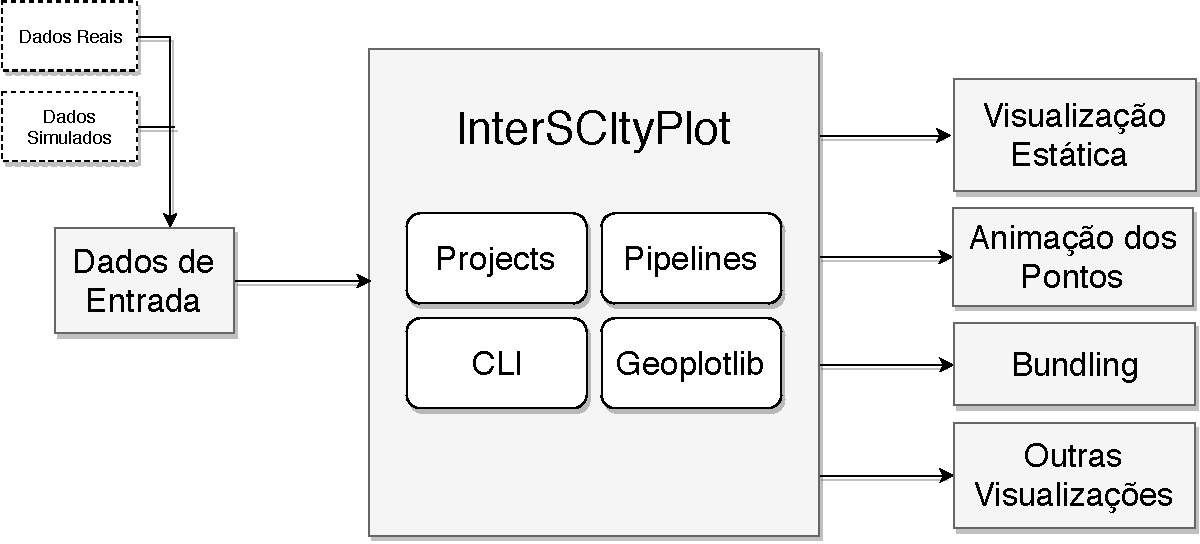
\includegraphics[width=1\textwidth]{../figuras/interscityplot.pdf}
  \caption{Visão geral da arquitetura da ferramenta InterSCityPlot que permite a criação
de múltiplas visualizações de dados geoespaciais.}
  \label{fig:interscityplot}
\end{figure}

\begin{description}
  \item[\emph{Projects}:] A exploração de dados do tráfego começa com a criação de um
novo projeto de visualização a partir de um conjunto de dados de entrada. Esse
componente é responsável pela criação, exclusão e outras ações de gerenciamento
dos projetos.

  \item[\emph{Pipelines}:] Os dados de entrada podem passar por uma ou mais
etapas de pré-processamento do módulo \emph{Pipelines} antes de serem
visualizados. Uma etapa padrão pela qual passam todos os projetos no momento de
sua criação é uma análise inicial que contabiliza o número de trajetórias,
quantidade média de pontos por trajetória e número total de pontos no conjunto
de dados fornecido. Outras etapas de pré-processamento podem ser adicionadas
conforme novas necessidades surgem, como por exemplo, limpeza dos dados para
checagem de inconsistências, derivação de novos atributos nos dados, etc.

  \item[Geoplotlib:] A biblioteca Geoplotlib, apresentada em
\citet{Andrea2016}, fornece recursos para criação de visualizações de dados
geoespaciais. Ela fornece todo o arcabouço em baixo nível para renderização de
imagens a partir desses dados e possui também algumas visualizações
pré-definidas para projetar pontos e linhas em um mapa.  Estendemos os recursos
desta biblioteca dentro do InterSCityPlot para a implementação da visualização
proposta.

  \item[CLI:] O módulo CLI possui a lógica para interação com a ferramenta
através da linha de comando. Essa interação se resume atualmente a comandos de
gerenciamento dos projetos (criação, exclusão) e execução de uma das
visualizações já desenvolvidas. A documentação completa pode ser vista no
repositório da ferramenta, disponível no
Github\footnote{\rurl{github.com/tallysmartins/interscity-plot}}.

\end{description}
